\documentclass[a4papaer,12pt]{article}
\usepackage{geometry}
\usepackage{titling}
\usepackage{indentfirst}
\usepackage{enumitem}
\renewcommand\maketitlehooka{\null\mbox{}\vfill}
\renewcommand\maketitlehookd{\vfill\null}
\usepackage{graphicx}
\graphicspath{ {./images/} }
\begin{document}

\begin{titlepage}
\sloppy
\begin{center}
BABE\c S BOLYAI UNIVERSITY, CLUJ NAPOCA, ROM\^ ANIA

FACULTY OF MATHEMATICS AND COMPUTER SCIENCE

\vspace{6cm}

\Huge \textbf{COR MEUM}

\vspace{1cm}

\normalsize -- MIRPR report --

\end{center}


\vspace{2cm}

\begin{flushright}
\Large{\textbf{Team members}}\\
Matei Sergiu Razvan, info romana, 235\\
Mardaloescu Ana-Maria, info romana, 235\\
Marian Andrada, info romana, 235\\
Molnar Radu-Stefan, info romana, 235
\end{flushright}

\vspace{2cm}

\begin{center}
2019
\end{center}

\end{titlepage}
\pagenumbering{arabic}


\section{Descrierea aplicației}
Un student la medicină dispune de o aplicație care îi prezintă vizual informații relevante despre inimă și malformațiile investigate și îl ajută să învețe despre acestea. Astfel, plecând de la informații preluate în format MRI, aplicația permite vizualizarea 3D a inimii, precum si a unor defecte posibile. 
\\
\indent Vizualizând imaginea 3D (încărcată de către student) studentul poate verifica dacă există sau nu malformații ale inimii, iar dacă da, atunci identificarea acesteia prin încercuire. La final, aplicația îi evidențiază malformația.

\section{Flow-ul aplicației}
Se pornește aplicația, se alege opțiunea de încărcare a imaginii în format nifti (.nii). Se încarcă imaginea și se dă check de către utilizator dacă acesta consideră ca inima din imagine prezintă malformații sau nu. Se transmite imaginea unui server unde se aplică un algoritm inteligent ce detectează malformația, după care este transformată în format 3D și trimisă inapoi la interfața cu utilizatorul, acesta având posibilitatea incarcarii unei noi imagini.

\section{Descrierea plastică a problemei}
Pe baza unei imagini (MRI) a unei inimi se aceasta prezinta una dintre cele doua cazuri: cazul normal sau cazul hypertrophic cardiomyopathy analizand imaginea la nivelul pixelilor.


\section{Descrierea formală a problemei}
Dezvoltarea unui algoritm ce realizează clasificarea inimilor dintr-o imaginea MRI in cadrul a doua clase: normal case si hypertrophic cardiomyopathy case. \\
\indent Algoritmul analizeaza inima cu ajutorul unei retele CNN si determina daca inima este una sanatoasa sau nu.

\section{Descrierea algoritmului}
Am dezvoltat un algoritm ce foloseste un CNN(Convolutional neural network) deoarece acesta este mai eficient decat o retea neuronala clasica cand vine vorba de imagini(o imagine de 100x100, adica o matrice de 100x100, are 10000 de weight-uri pentru stratul 2). Operatia de convolutie consta in luarea unei sectiuni(3x3) din imagine() si aplicarea unei functii pe acea zona rezultatul urmand sa fie valoarea zonei. Polling-ul este o operatie a CNN care consta in luarea unei zone din matrice(2x2) si alegerea valorii maxime din acea zona pentru a forma noua matrice rezultat.CNN-ul are 3 straturi convolutionale 3x3 cu functii relu de activare, si 2 straturi de pooling de tip max, 2x2. 

\section{Descrierea Metodologiei}
Faza 1:
S-a folosit modelul secvential (stiva de straturi) impreuna cu 3 straturi Conv2D, fiecare cu filtre 64, dimensiunea pooling-ului de (3,3), functia de activare 'relu'. Pentru straturile de pooling s-a folosit MaxPooling2D cu dimensiune de (2,2). In final s-au adaugat 2 straturi Dense cu functia de activare 'relu' respectiv 'softmax'. 
S-au folosit 56 date de train, impartite in 4 categorii si 5 date de train. Datele au fost prelucrate folosind pickle. Pentru 3 epoci s-a obtinut o acuratete de 0.3 si un loss de 2.98. In cazul a 5 epoci s-a obtinut o acuratete de 0.44 si un loss de 1.42. Pentru cazuri cu 10 epoci algoritmul face overfitt, acuratetea fiind 1, iar loss-ul 0.03.
Posibile cauze: s-a presupus ca rezultatele ar putea fi influentate de neuniformizarea datelor, acestea fiind 'alese' asftel incat sa nu fie necesara interpolarea (date cu aceeasi dimensiune z) sau de numarul redus al acestora.
Pentru 50 de date din 4 categorii dintre care s-au ales 10 pentru test, s-a obtinut un rezultat de 0,20 acuratete. Algoritmul a rulat pentru 2, 5 si 10 epoci, obtinand rezultate mai proste cu cat mai multe epoci rula. 

Faza 2:
S-a incercat prelucrarea datelor in mod diferit, fara normalizare, dar cu o retea care sa primeasca ca si input 4 parametri fara constrangeri. La rularea algoritmului acesta se opreste in faza de train datorita memoriei prea putine.

Faza 3:
S-a reusit o redimensionare a imaginii prin interpolare de tip "nearest" astfel incat datele sa aiba aceeasi dimensiune. Pentru antrenament am folosit 120 de date, impartite echitabil in cele 5 categorii. Pentru test s-au folosit 20 de date, pentru care s-a obtinut o acuratete de 0.6 si loss de 0.86, in cazul a 5 epoci. 
\\
Pentru 70 de epoci si aceleasi date s-a obtinut acuratete de 0.95 
si un loss de 0.06.
\newpage
\section{Architecture}

\indent \textbf{CNN-Layers:}
\\
\\
\begin{tabular}{|c|c|c|c|c|c|}
	\hline
	Layer & Type & Convolution & Channels & Stride & Options on layer\\
	\hline
	1 & convolutional & 3x3 & 32 & - & - \\
	\hline
	2 & pooling & - & - & 2x2 & max \\
	\hline
	3 & convolutional & 3x3 & 64 & - & - \\
	\hline
	4 & pooling & - & - & 2x2 & max \\	
	\hline
	5 & convolutional & 3x3 & 64 & - & - \\
	\hline
	6 & flatten & - & - & - & -\\	
	\hline
	7 & relu & - & - & - & 64 \\
	\hline
	8 & softmax & - & - & - & 10\\
	\hline
\end{tabular}
\\
\\
\indent \textbf{Project-UML-Diagram:}
\\
\\
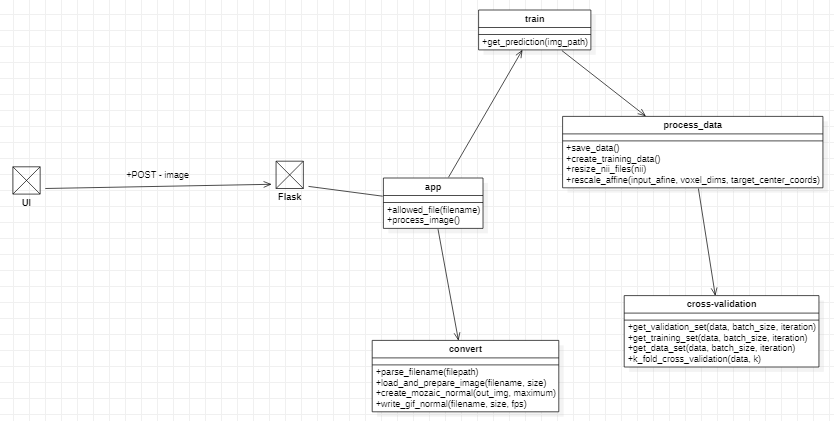
\includegraphics[scale=0.75]{diagrama.png}

\section{Testing Metrics}
Number of training data: 120
\\
Number of test data: 25
\\
Loss: sparse categorical crossentropy
\\
Optimizer: adam
\\

\begin{tabular}{|c|c|c|}
	\hline
	Metrics & Result Accuracy & Results loss \\
	\hline
	Accuracy & 0.62 & 0.73 \\
	\hline
	Binary Accuracy & 0.08 & 0.77 \\
	\hline
	Categorical Accuracy & 0.12 & 0.94 \\
	\hline
	Sparse Categorical Accuracy & 0.5 & 0.99 \\	
	\hline
	Top k Categorical Accuracy & 0.5 & 0.89 \\
	\hline
\end{tabular}
\\\\
Accuracy - statistics
\\
Benchmark tests
\\
Number of training data: 25
\\
Number of test data: 5
\\
\\
\begin{tabular}{|c|c|c|}
	\hline
	Epochs & Accuracy & Loss \\
	\hline
	5 & 1.0 & 0.47 \\
	\hline
	10 & 0.80 & 0.34 \\
	\hline
	15 & 0.80 & 0.23 \\
	\hline
	20 & 1.0 & 0.13 \\	
	\hline
	25 & 1.0 & 0.14 \\
	\hline
\end{tabular}

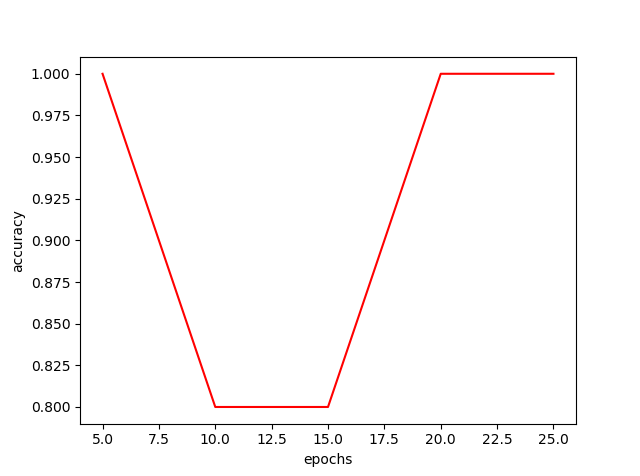
\includegraphics[scale=0.5]{Accuracy-Epoch-Benchmark.png}
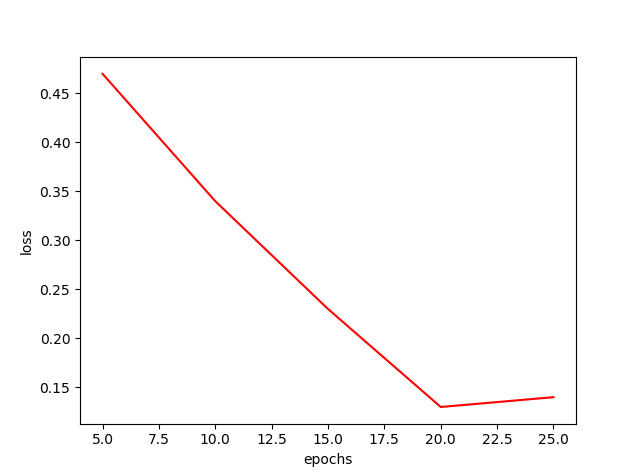
\includegraphics[scale=0.5]{Loss-Epochs-Benchmark.png}
\\
\indent \textbf{Real tests}
\\
Number of training data: 120
\\
Number of test data: 24
\\
\\
\begin{tabular}{|c|c|c|}
	\hline
	Epochs & Accuracy & Loss \\
	\hline
	5 & 0.45 & 1.10 \\
	\hline
	10 & 0.54 & 1.01 \\
	\hline
	15 & 0.54 & 1.00 \\
	\hline
	20 & 0.45 & 1.02 \\	
	\hline
	25 & 0.70 & 0.94 \\
	\hline
	30 & 0.62 & 1.03 \\	
	\hline
	35 & 0.79 & 0.88 \\
	\hline
	40 & 0.80 & 0.62 \\	
	\hline
	45 & 0.83 & 0.58 \\
	\hline
	50 & 0.79 & 0.56 \\	
	\hline
	55 & 0.79 & 0.48 \\
	\hline
	60 & 0.91 & 0.28 \\	
	\hline
	65 & 0.85 & 0.21 \\
	\hline
	70 & 0.87 & 0.25 \\	
	\hline
	75 & 0.95 & 0.11 \\
	\hline
	80 & 0.91 & 0.37 \\	
	\hline
	85 & 0.95 & 0.11 \\
	\hline
	90 & 0.95 & 0.05 \\	
	\hline
	95 & 0.95 & 0.06 \\
	\hline
	100 & 0.95 & 0.03 \\	
	\hline
\end{tabular}
\\
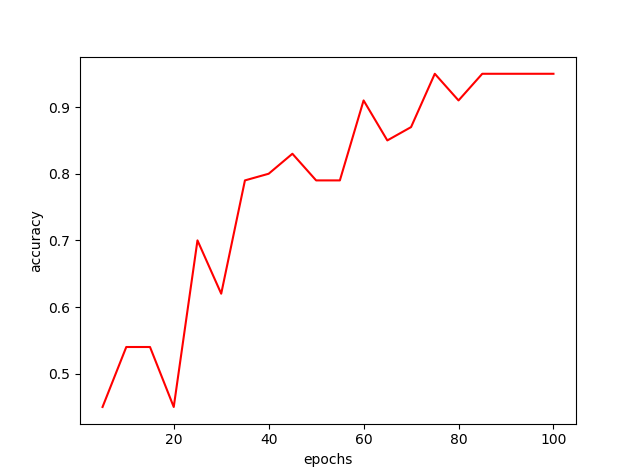
\includegraphics[scale=0.5]{Accuracy-Epochs.png}
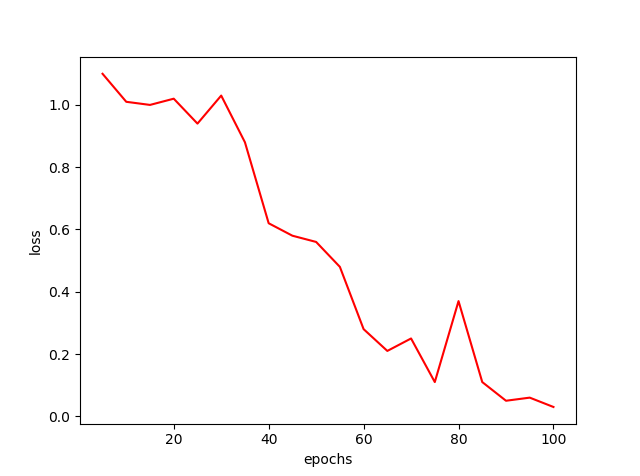
\includegraphics[scale=0.5]{Loss-Epochs.png}


\indent \textbf{Cross-validation results}
\\
\\
\begin{tabular}{|c|c|c|}
	\hline
	Epochs & Accuracy & Loss \\
	\hline
	10 & 0.45 & 1.10 \\
	\hline
	20 & 0.54 & 1.01 \\
	\hline
	30 & 0.54 & 1.00 \\
	\hline
	40 & 0.45 & 1.02 \\	
	\hline
	50 & 0.70 & 0.94 \\
	\hline
	60 & 0.62 & 1.03 \\	
	\hline
	70 & 0.79 & 0.88 \\
	\hline
	80 & 0.80 & 0.62 \\	
	\hline
	90 & 0.83 & 0.58 \\
	\hline
	100 & 0.79 & 0.56 \\		
	\hline
\end{tabular}

\section{Future work}

Pe viitor, ne-am propus sa introducem o parte de segmentare cardiovasculara care sa poata detecta malformatia pe baza unor cunostinte anterioare si vizualizarea acesteia, precum si segmentarea celor 4 zone ale inimii si vizualizarea acestora. 
\newpage

\section{Related work}
Fiecare student a căutat alte studii făcute în domeniu, care ar putea fi utile la realizarea acestui proiect.

\subsection{Ana}

\textbf{Titlul studiului} : \begin{Large}
Four-Chamber Heart Modeling and Automatic Segmentation for 3D Cardiac CT Volumes Using Marginal Space Learning and Steerable Features
\end{Large}
\\\\
\indent \textbf{Realizatori} : \begin{large}
Yefeng Zheng, Adrian Barbu, Bogdan Georgescu, Michael Scheuering, and Dorin 
Comaniciu
\end{large}
\\\\
\indent \textbf{Date} : 457 de volume cu cele 4 camere etichetate manual, provenite de la 186 de pacienți cu diferite boli cardiovasculare
\\\\
\indent \textbf{Algoritmi folosiți} : marginal space learning (MSL) și steerable features.
\\\\
\indent \textbf{Concluzii și rezultate} : o viteză medie de 4 secunde per volum pentru segmentarea celor 4 camere. Abordare generală de segmentare– se poate aplica pe mai multe organe. 


\subsection{Andrada}

\textbf{Titlul studiului} : \begin{Large}
Deep Learning Techniques for Automatic MRI
Cardiac Multi-structures Segmentation and
Diagnosis: Is the Problem Solved?
\end{Large}
\\\\
\indent \textbf{Realizatori} : \begin{large}Olivier Bernard, Alain Lalande, Clement Zotti, Frederick Cervenansky, Xin Yang, Pheng-Ann Heng, Irem Cetin,
Karim Lekadir, Oscar Camara, Miguel Angel Gonzalez Ballester, Gerard Sanroma, Sandy Napel,
Steffen Petersen, Georgios Tziritas, Elias Grinias, Mahendra Khened, Varghese Alex Kollerathu,
Ganapathy Krishnamurthi, Marc-Michel Rohe, Xavier Pennec, Maxime Sermesant, Fabian Isensee, Paul Jager,
Klaus H. Maier-Hein, Peter M. Full, Ivo Wolf, Sandy Engelhardt, Chrisitan F. Baumgartner, Lisa M. Koch,
Jelmer M. Wolterink, Ivana Isgum, Yeonggul Jang, Yoonmi Hong, Jay Patravali, Shubham Jain, Olivier Humbert,
and Pierre-Marc Jodoin
\end{large}
\\\\
\indent \textbf{Date} : Datele de antrenament au fost furnizate de ACDC (Automatic Cardiac Diagnosis Challenge), 70 de imagini MRI cu inimi sănătoase și 30 cu inimi bolnave, iar datele de test au fost 50 imagini MRI 
\\\\
\indent \textbf{Algoritmi folosiți} : Isensee a folosit o serie de atribute dinamice folosind o rețea neuronală cu 50 de multi-layere, iar pentru clasificare a folosit random forest 
\\\\
\indent \textbf{Concluzii și rezultate} : Ca și rezultat s-a obținut o acuratețe de 0.92.


\subsection{Sergiu}

\textbf{Titlul studiului} : \begin{Large}
Screening for cardiac contractile dysfunction using an artificial intelligence–enabled electrocardiogram
(Funcția contractilă a miocardului)
\end{Large}
\\\\
\indent \textbf{Realizatori} : \begin{large} Zachi I. Attia, Suraj Kapa, Francisco Lopez-Jimenez, Paul M. McKie, Dorothy J. Ladewig, Gaurav Satam, Patricia A. Pellikka, Maurice Enriquez-Sarano, Peter A. Noseworthy, Thomas M. Munger, Samuel J. Asirvatham, Christopher G. Scott, Rickey E. Carter \& Paul A. Friedman 
\end{large}
\\\\
\indent \textbf{Date} : S-au folosit datele electrocardiogramelor a 44.959 pacienți ai clinicii Mayo pentru antrenare, care conțineau date și despre fracţia de ejecţie a ventriculului stâng. Testarea s-a făcut pe 52.870 de pacienți
\\\\
\indent \textbf{Algoritmi folosiți} : Clasificare folosind CNN , funcția de predicție definită ca fracția de ejecție <= 35%
\\\\
\indent \textbf{Concluzii și rezultate} : Pe setul de test acuratetea a fost de 85.7\%, specificitate de 85.7\%, senzitivitate de 86.3\% si AUC de 0.93
\\\\

\subsection{Radu}

\textbf{Titlul studiului} : \begin{Large}\begin{enumerate}[label=\Roman*, font=\bfseries]
\item Dilated convolutional neural networks for cardiovascular MR segmentation in congenital heart disease, 2017
\item Automated cardiovascular segmentation in patients with congenital heart disease from 3D CMR scans: Combining multi-atlases and level-sets, 2017
\end{enumerate}
\end{Large}

\indent \textbf{Realizatori} : \begin{large}\begin{enumerate}[label=\Roman*, font=\bfseries]
\item Jelmer M. Wolterink, Tim Leiner, Max A. Viergever and Ivana Isgum
\item Rahil Shahzad, Shan Gao, Qian Tao, Oleh Dzyubachyk and Rob van der Geest
\end{enumerate}
\end{large}

\indent \textbf{Date} : HVSMR 2016 MICCAI challenge organizer
\\\\
\indent \textbf{Algoritmi folosiți} : O primă metodă pentru împărțirea inimii din imagine și pentru determinarea părților ei se poate folosi o segmentare tip atlas-based pentru învățarea zonelor pe baza unor cunoștințe anterioare(se poate folosi un gradient descrescător pentru potrivirea atlasului cu cea a imaginii). Pentru detecția mușchiului miocard se poate folosi o clusterizare cu 2 clase una pentru sânge iar cealaltă pentru mușchi. Această împărțire ne poate ajuta la determinarea bolilor congenitale.
\indent O a doua metodă găsită pentru rezolvarea acestei probleme ar fi folosirea unei rețele neuronale convoluțională. O astfel de rețea este perfectă pentru procesarea de imagini. Aceasta va fi antrenată să determine vasele de sânge și mușchiul miocard.
\\\\
\indent \textbf{Concluzii și rezultate} :
\\ 
\indent Metoda 1: Dice index de 0.89 pentru vasele de sânge și 0.75 pentru țesuturile miocardice.
\\
\indent Metoda 2: Dice index de 0.93 pentru vasele de sânge și 0.80 pentru țesuturile miocardice

\end{document}